\documentclass[10pt,a4paper]{article}
\usepackage[utf8]{inputenc}
\usepackage{amsmath}
\usepackage{amsfonts}
\usepackage{amssymb}
\usepackage{listings}
\usepackage{graphicx}
\lstset{showstringspaces=false,
		breaklines=true,
		postbreak=\raisebox{0ex}[0ex][0ex]{\ensuremath{\hookrightarrow\space}}}
    	
\begin{document}
\title{Intelligent Systems Assignment 2}
\author{Wessel Becker (1982362) \& Sander ten Hoor (2318555)}
\maketitle

\section{Matlab Code}
The following code was created to obtain the plots.

\subsection{main.m}
\lstinputlisting[language=Matlab]{./VQ/main.m}

\subsection{changeDistance.m}
\lstinputlisting[language=Matlab]{./VQ/changeDistance.m}

\subsection{randomDataPoints.m}
\lstinputlisting[language=Matlab]{./VQ/randomDataPoints.m}

\subsection{vectorQuantization.m}
\lstinputlisting[language=Matlab]{./VQ/vectorQuantization.m}

\subsection{euclidean.m}
\lstinputlisting[language=Matlab]{./VQ/euclidean.m}

\subsection{vectorQuantization.m}
\lstinputlisting[language=Matlab]{./VQ/vectorQuantization.m}	

\subsection{quantizationError.m}
\lstinputlisting[language=Matlab]{./VQ/quantizationError.m}

\subsection{plotVQ.m}
\lstinputlisting[language=Matlab]{./VQ/plotVQ.m}

\subsection{plotLearningCurve.m}
\lstinputlisting[language=Matlab]{./VQ/plotLearningCurve.m}

\section{Plots}
For plotting, dataset x was chosen. The values for the learning rate were 0.1, 0.01 and 0.001. They are included at the end of this document.

\section{Discussion}
In the discussion the results of, running this simple VQ algorithm for different learning rates and with different numbers of prototypes are discussed. We will focus on the influence of the learning rate on the obtained result but also mention some other interesting observations.

\subsection{Fluctuation}
\label{subsec:fluc}
At higher learning rates, the quantization error fluctuates a lot more than at lower learning rates, for which the graph are smoother, see figures \ref{fig:n01_k2_learning}, \ref{fig:n001_k2_learning} and \ref{fig:n0001_k2_learning} for an example. This effect is caused by the higher movement at higher learning rates. Which make the solutions cause the most recently evaluated data points die be more influential to the chosen values for the prototype vectors. Since the prototypes will change allot towards this points. At lower values for the learning rate the prototype vectors will evaluate single data points less strongly and therefore tend to stay more related to all data points to which it is closest.

\subsection{Number of prototypes}
\label{subsec:numpro}
When the number of prototypes is higher, the learning process is slower. This is because every time the distance is evaluated, still only one prototype is updated. If the number of prototypes is twice as large as before, the learning speed for each individual prototype is cut in half.

\subsection{Run time versus optimal result}
At higher learning rates the algorithm reaches a minimum much faster then at lower learning rates, see for example figures \ref{fig:n01_k4_learning} and \ref{fig:n0001_k4_learning} for a difference. Which means that a good solution could be found in a much smaller time frame. Sadly, this faster learning speed comes at the cost of having a less stable result which could mean a less optimal solution as was discussed in \ref{subsec:fluc}. This means that in practice we will need to make a choice for the learning rate that balances these to factors, keeping in mind the influence of adding more prototypes, see \ref{subsec:numpro}.

\subsection{Winner takes all}
In one of the plots, there are three prototypes in one half, and one in the other. This affects the quantization error, which might be lower if there were two prototypes on each side. However, this state is never achieved because only the winner is updated. In the right half, the winner is always the sole prototype there. This means the algorithm could easily get stuck in a local minimum.

\section{Work done}
For this assignment, the algorithm implementation was done by Wessel, while Sander worked on plotting. The latter created the plots and put together this document, after which Wessel made some suggestions and modifications.

\begin{figure}
  \centering
    \makebox[\textwidth]{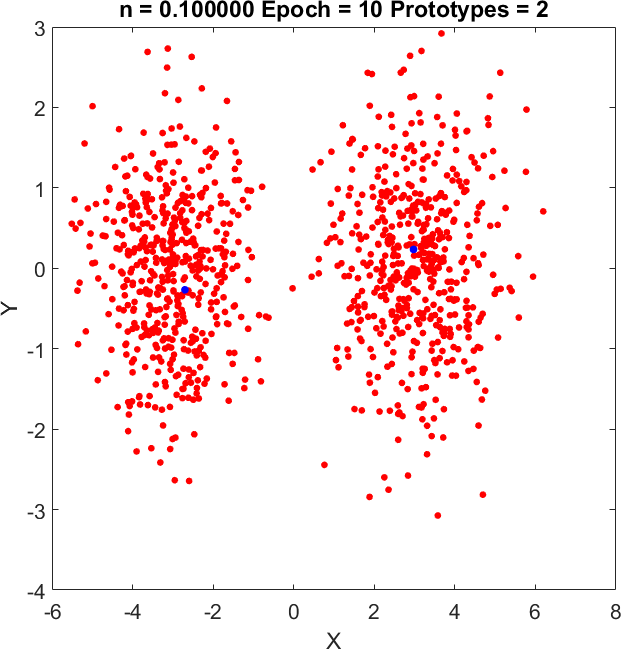
\includegraphics[width=\textwidth]{./VQ/x_e10_n01_k2}} \\
  \caption{Scatter, n = 0.1, 2 prototypes}
  \label{fig:n01_k2}
\end{figure}

\begin{figure}
  \centering
\makebox[\textwidth]{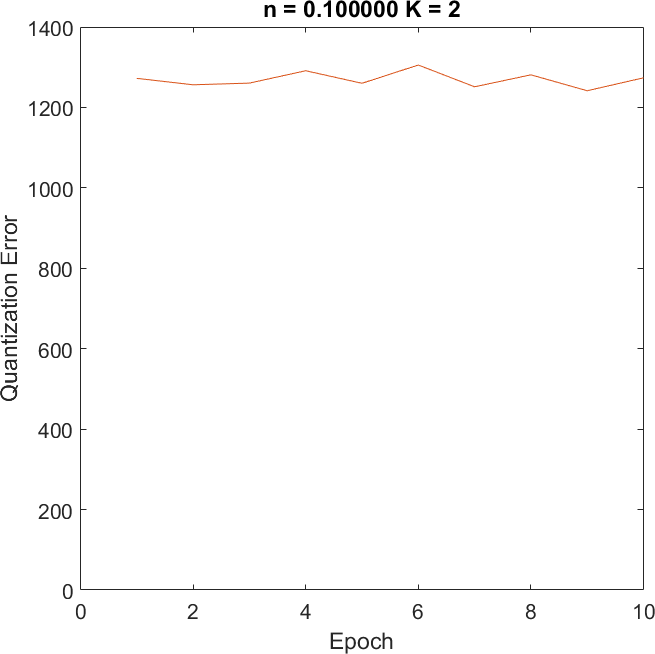
\includegraphics[width=\textwidth]{./VQ/x_e10_n01_k2_learning}} \\
  \caption{Quantization Error, n = 0.1, 2 prototypes}
  \label{fig:n01_k2_learning}
\end{figure}

\begin{figure}
  \centering
\makebox[\textwidth]{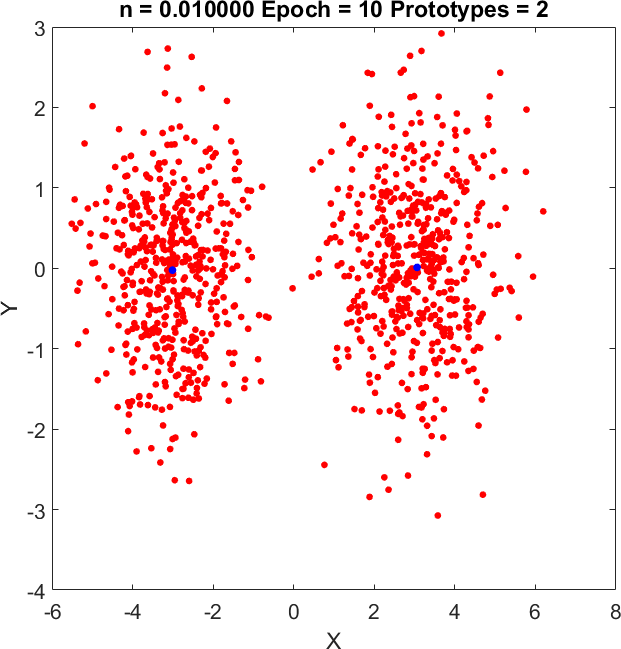
\includegraphics[width=\textwidth]{./VQ/x_e10_n001_k2}} \\
  \caption{Scatter, n = 0.01, 2 prototypes}
  \label{fig:n001_k2}
\end{figure}

\begin{figure}
  \centering
\makebox[\textwidth]{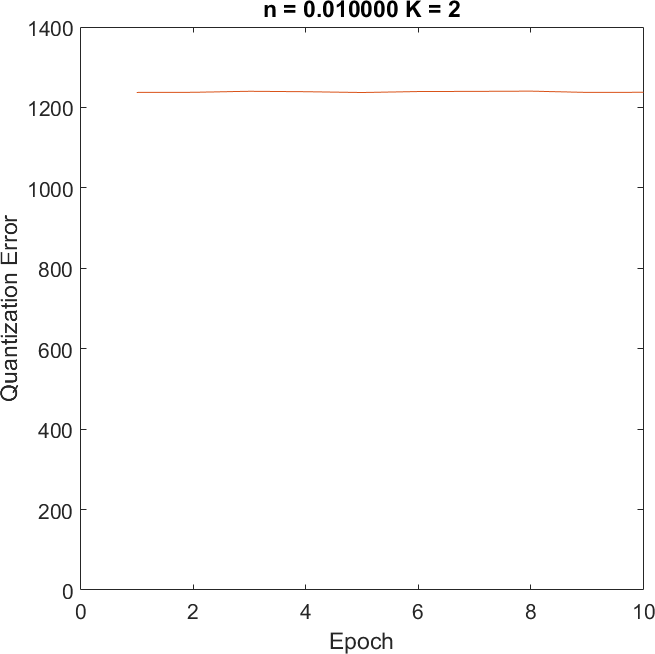
\includegraphics[width=\textwidth]{./VQ/x_e10_n001_k2_learning}} \\
  \caption{Quantization Error, n = 0.01, 2 prototypes}
  \label{fig:n001_k2_learning}
\end{figure}

\begin{figure}
  \centering
\makebox[\textwidth]{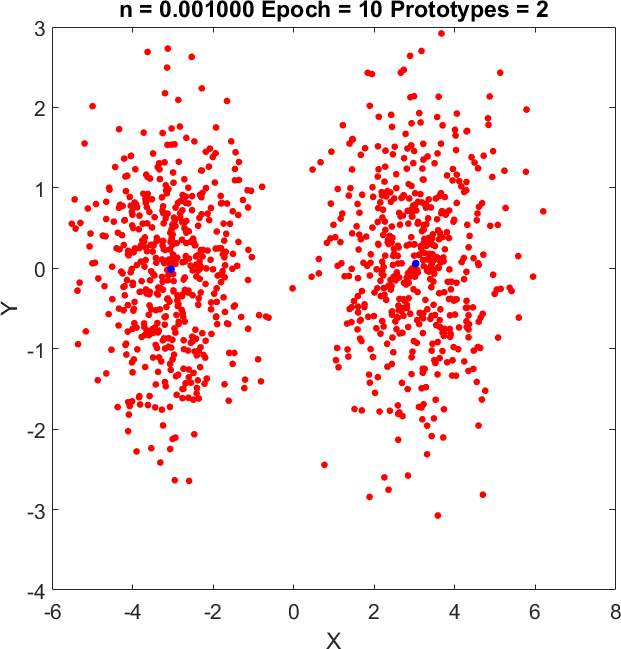
\includegraphics[width=\textwidth]{./VQ/x_e10_n0001_k2}} \\
  \caption{Scatter, n = 0.001, 2 prototypes}
  \label{fig:n0001_k2}
\end{figure}

\begin{figure}
  \centering
\makebox[\textwidth]{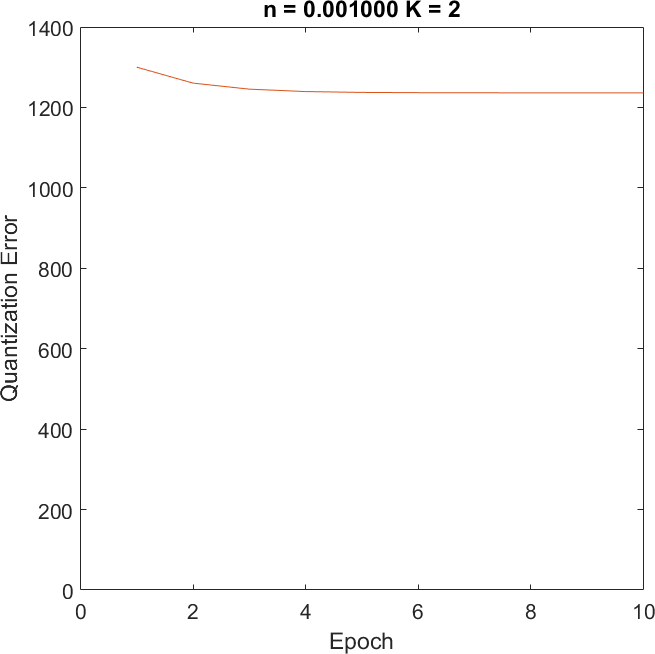
\includegraphics[width=\textwidth]{./VQ/x_e10_n0001_k2_learning}} \\
  \caption{Quantization Error, n = 0.001, 2 prototypes}
  \label{fig:n0001_k2_learning}
\end{figure}

\begin{figure}
  \centering
\makebox[\textwidth]{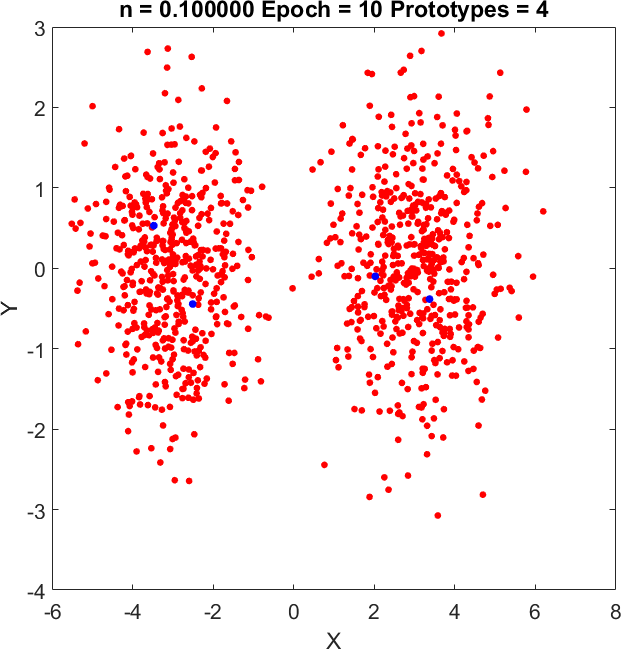
\includegraphics[width=\textwidth]{./VQ/x_e10_n01_k4}} \\
  \caption{Scatter, n = 0.1, 4 prototypes}
  \label{fig:n01_k4}
\end{figure}

\begin{figure}
  \centering
\makebox[\textwidth]{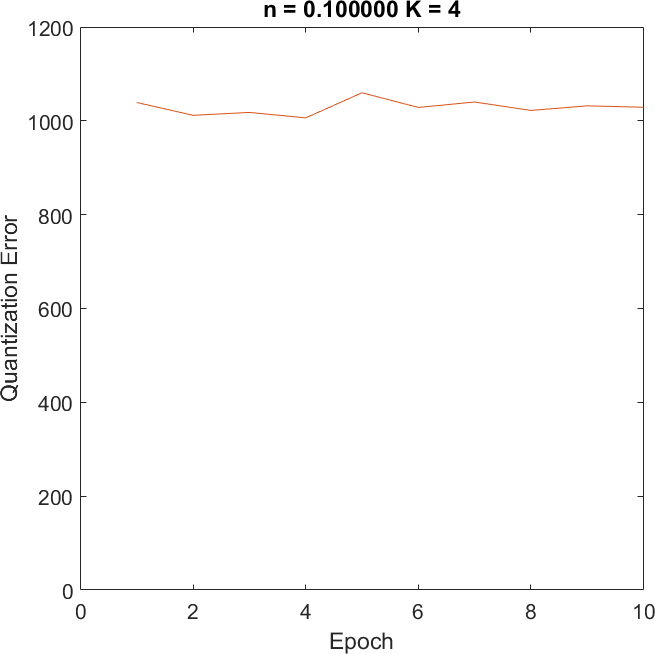
\includegraphics[width=\textwidth]{./VQ/x_e10_n01_k4_learning}} \\
  \caption{Quantization Error, n = 0.1, 4 prototypes}
  \label{fig:n01_k4_learning}
\end{figure}

\begin{figure}
  \centering
\makebox[\textwidth]{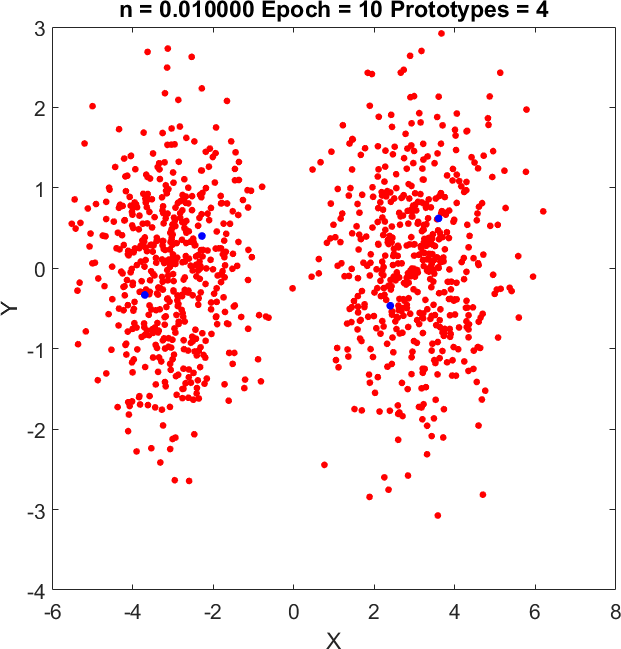
\includegraphics[width=\textwidth]{./VQ/x_e10_n001_k4}} \\
  \caption{Scatter, n = 0.01, 4 prototypes}
  \label{fig:n001_k4}
\end{figure}

\begin{figure}
  \centering
\makebox[\textwidth]{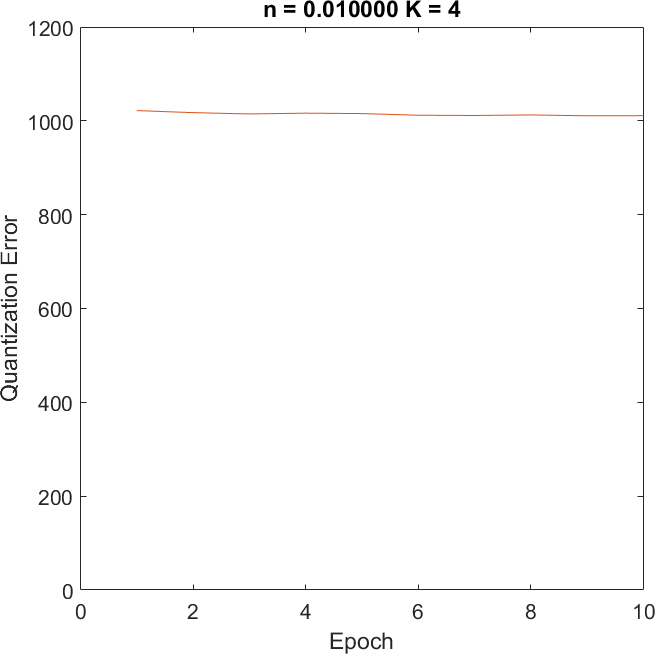
\includegraphics[width=\textwidth]{./VQ/x_e10_n001_k4_learning}} \\
  \caption{Quantization Error, n = 0.01, 4 prototypes}
  \label{fig:n001_k4_learning}
\end{figure}

\begin{figure}
  \centering
\makebox[\textwidth]{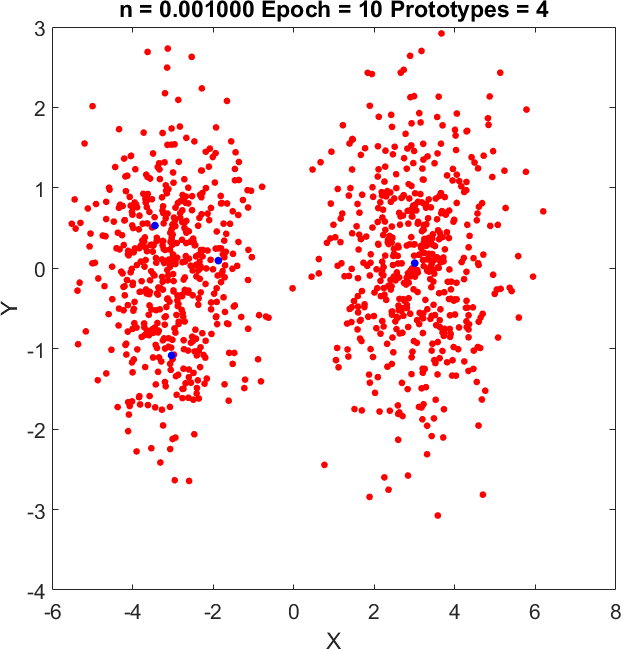
\includegraphics[width=\textwidth]{./VQ/x_e10_n0001_k4}} \\
  \caption{Scatter, n = 0.001, 4 prototypes}
  \label{fig:n0001_k4}
\end{figure}

\begin{figure}
  \centering
\makebox[\textwidth]{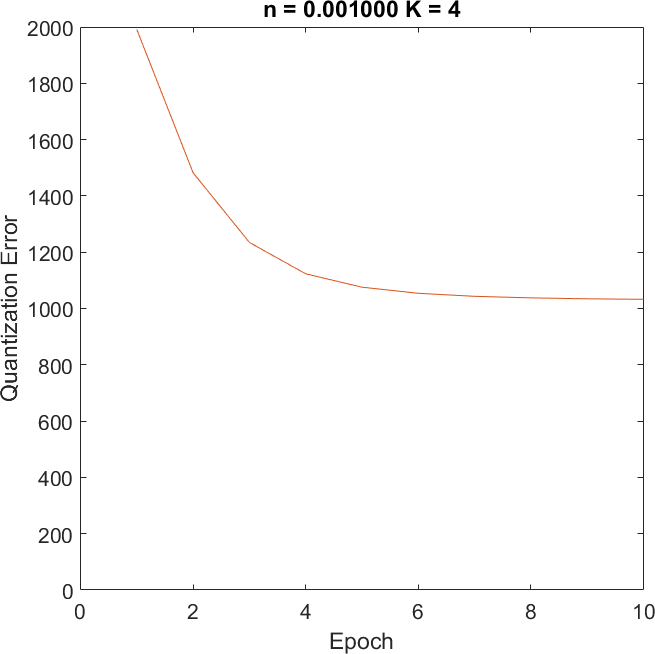
\includegraphics[width=\textwidth]{./VQ/x_e10_n0001_k4_learning}} \\
  \caption{Quantization Error, n = 0.001, 4 prototypes}
  \label{fig:n0001_k4_learning}
\end{figure}
\end{document}